\documentclass[12pt]{article}
\usepackage{amsfonts,amssymb}
\usepackage{exercise}
\usepackage{amsmath}
\usepackage{amsthm}
\usepackage{hyperref}
\usepackage{graphicx}
\usepackage{listings}
%\documentstyle[12pt,amsfonts]{article}
%\documentstyle{article}

\setlength{\topmargin}{-.5in}
\setlength{\oddsidemargin}{0 in}
\setlength{\evensidemargin}{0 in}
\setlength{\textwidth}{6.5truein}
\setlength{\textheight}{8.5truein}
%
%\input ../adgeomcs/lamacb.tex
%\input ../mac.tex
%\input ../mathmac.tex
%
\input xy
\xyoption{all}
\def\fseq#1#2{(#1_{#2})_{#2\geq 1}}
\def\fsseq#1#2#3{(#1_{#3(#2)})_{#2\geq 1}}
\def\qleq{\sqsubseteq}
\newtheorem{theorem}{Theorem}
%cis51109hw1

%
\begin{document}
\begin{center}
\fbox{{\Large\bf Introduction to Induction}}\\
\vspace{1cm}
\end{center}

\vspace{0.5cm}\noindent


\section*{Recognizing a pattern}

Consider the following pattern

\begin{align*}
 1 + 3 &= 4 \\
 1 + 3 +  5 &= 9 \\
 1 + 3 + 5 + 7 &= 16
\end{align*}


The pattern at this point is hopefully becoming clear. Let us do one more

$1 + 3 + 5 + 7 + 9 = 25$

Looks like the sum of odd numbers is equal to some perfect square. It is time to formalize this.
Every odd number is of the form $2k + 1$ for some integer $k$. That should lead us to this

\begin{align*}
\sum_{i=1}^n 2i - 1 = n^2
\end{align*}

where $n \in \mathbb{N}$.

Whenever you have a result that follows a pattern like this, in order to prove it you have to show the formula/pattern holds for every single value of $n$. Since $n$ takes values in `discrete' steps (1,2,3 etc), the powerful method called induction can be applied to prove it.
 
\section*{Idea behind induction}
Induction is used to prove that a theorem holds for all natural numbers (sometimes we will include 0). 

If we are able to show the following. 

\begin{itemize}
\item the theorem holds for 1 (or some small number)
\item If the theorem holds for $n-1$, then it will hold for $n$.
\end{itemize}

Now let's say we want to show the theorem is going to hold for 5. Here's how we could do it

\begin{itemize}
\item it holds for 1
\item Since it holds for 1, it holds for 2.
\item Since it holds for 2, it holds for 3.
\item Since it holds for 3, it holds for 4.
\item Since it holds for 4, it holds for 5.
\end{itemize}

This idea of using the previous to prove the current is the crux of induction. If you have seen recursion in programming, this methodology of solving sub problems and using their solution to solve the big problem should look familiar. It is closely closely related to recursion. 

\section*{Outline of an induction proof}

\begin{enumerate}
\item Write the statement of the theorem in terms of a predicate that has an input of a single number.  Your goal in proving the result/theorem is to show the predicate will always return the value true regardless of what number is used as an input. So your theorem is now stated as 

To show P(n) is true for all positive n (or for all $n \ge 42$ or something like that) where P(n) is defined as ....

\item Prove the theorem for the smallest possible $n$. Generally this will be something like $0$ or $1$ but it depends on the theorem. This is called the base case.
\item Show $P(n-1) \implies P(n)$

Remember that to prove the above implication we need to assume $P(n-1)$ to be true and use that in some manner when we are proving $P(n)$.

It is common convention to call the $P(n-1)$ is true assumption the \emph{induction hypothesis}.

\end{enumerate}

\section*{Proof of summations}

Let us attempt an inductive proof of the first result.

\begin{align*}
\sum_{i=1}^n 2i - 1 = n^2
\end{align*}

Define the predicate $P(n)$ as a function which returns true or false depending 

Base case: When $n=1$, there is only term in the summation which is $ 2 - 1 = 1$ and the right side is also 1. So it is true for 1.

Assume the result is true for $n-1$ So 

\begin{align*}
\sum_{i=1}^{n-1} 2i - 1 = (n-1)^2
\end{align*}

To show if $P(n-1)$ then $P(n)$.

Consider the sum 

\begin{align*}
\sum_{i=1}^n 2i - 1 &= \sum_{i=1}^{n-1} 2i - 1 + 2n - 1 \\
&= (n-1)^2 + 2n - 1 \tag{using P(n-1) true}\\
&= n^2 - 2n + 1 + 2n - 1 \\
&= n^2
\end{align*}

which shows that the predicate is true for $n$.

\section*{Proof of inequalities}

Which is greater $n!$ or $2^n$? 

3! is 6 and $2^3$ is 8. 4! is 24 and $2^4$ is 16. 5! is 120 and $2^5=32$. So looks like the inequality $n! > 2^n$ holds for $n \ge 4$

To prove this claim by induction.

Let the predicate be defined as $n! > 2^n, n \ge 4$.

The base case is $n = 4$ which we have already shown to be true.

Let the statement hold true for $n-1$. Meaning 

\begin{equation} \label{eq:prop}
(n-1)! > 2^{n-1}
\end{equation}

To prove this inductively we need to use this to show $n! > 2^n$.

Multiply both sides of ~\ref{eq:prop} by $n$ since $n! = (n-1)!n$.

So we get $n! > 2^{n-1} \cdot n$. Since $n >4$, we know that 

$2^{n-1} \cdot n > 2^{n-1} \cdot 2$ 

But $2^{n-1} \cdot 2 = 2^n$

Hence proved

\section*{Example involving sets}

Generalized De-Morgan's law.

We will do this in class and the steps are all in the Zybook as part of participation activity 10.5.6

\section*{Induction puzzle}

 In Josephine's kingdom every woman has to pass a logic exam before being allowed to marry. Every married woman knows about the fidelity of every man in the kingdom except for her own husband, and etiquette demands that no woman should tell another about the fidelity of her husband. Also, a gunshot fired in any house in the kingdom will be heard in any other house. Queen Josephine announced that unfaithful men had been discovered in the kingdom, and that any woman knowing her husband to be unfaithful was required to shoot him at midnight following the day after she discovered his infidelity. How did the wives manage this?
 
This is a classic puzzle and the solution can actually be found on wikipedia. We will discuss in class or recitation.

\section*{Divisibility proof}

$2^{n+2} + 3^{2n+1}$ is divisible by 7 for all positive integers

Proof by induction

Let $P(n)$ be the predicate that returns true when $2^{n+2} + 3^{2n+1}$ is divisible by 7.

Base case: P(1) says $2^3 + 3^3 = 8 + 27 = 35$ and 35 is $5 \times 7$.

To show $P(n-1) \rightarrow P(n)$.

We are given that $2^{(n-1) + 2} + 3^{2(n-1)+1}$ is divisible by 7. That is $2^{n+1} + 3^{2n-1}$ is divisible by 7.

We now consider $2^{n+2} +3^{2n+1}$ and simplify it to the point where we can use our induction hypothesis and prove the theorem.

\begin{align*}
2^{n+2} + 3^{2n+1} \\
&= 2\cdot(2^{n+1} + 3^{2n-1}) + 3^{2n+1} - 2\cdot 3^{2n-1} \\
&= 2\cdot(2^{n+1} + 3^{2n-1}) + 3^{2n-1}(3^2 - 2) \\
&= 2\cdot(2^{n+1} + 3^{2n-1}) + 3^{2n-1}\cdot 7 
\end{align*}

The first term is divisible by 7 because of the induction hypothesis. The second term is clearly divisible by 7.

Hence we have shown that $P(n-1) \rightarrow P(n)$, which along with the base case completes a proof by induction.

\section*{Breaking down or building up}

The most controversial aspect of induction happens to be whether to build the problem up or break the problem down. It is universally true that breaking the problem down is the correct way to go. The issue is that in a lot of the algebraic questions, building the problem up works as well. So it is easy to fall into the trap of using that as your approach always. 

The place where this concept of building the problem up definitely breaks down is actually closer to computer science which is the reason for stressing it so much.

\subsection*{Autocities}

One example of the build up versus breaking down aspect of induction proofs is the following

Define an autocity to be a city that has a road that leads to some other(different) city. 

Claim: In any collection of $n$ autocities there is a way (obviously via a collection of roads) to get from any city to any other city.

Let us try a proof by induction

Base case: We need at least 2 cities for the definition of autocity to work. With 2 cities, the only way that both of them can be autocities is if there is a road connecting them. So the statement of the claim is obviously true when we have 2 cities.

Induction hypothesis: In any collection of $n-1$ autocities there is a path between any pair of cities.

Now consider adding in the $n$th city. For this city to be an autocity, it must be connected via a road to one of these $n-1$ autocities. Now consider any pair of autocities in this collection of $n$. If the pair comes from the previous $n-1$ cities there is a path via the induction hypothesis. If the pair includes the newly added city, we can use a road to get from the $n$th city to whatever city it was connected to. Let's call that $D$. Then there is a path from $D$ to any other city (by the induction hypothesis). So now we have a path between any pair of cities. Hence proved.

Seemingly we have proven by induction.

But let us step back and see if the claim is true. It isn't. See below!

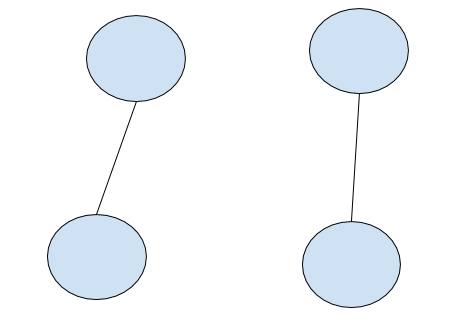
\includegraphics[scale=0.5]{./img/autocity.png}

Try doing this same proof by taking  any collection of $n$ autocities and removing an autocity. You will find that it is impossible to make the claim that by removing an autocity you still have a collection of autocities. So by the breaking down method you will not run into an incorrect proof.


Consider the example of the following question

\begin{Exercise*}
Prove that in a group of N people,
if some of them shake hands,
there are at least two who have the same number of handshakes. 
\end{Exercise*}

The solution offered at the \href{http://www.gottfriedville.net/mathprob/comb-shakes.html}{website} has a number of issues but the biggest amongst them is that it assumes that `a person enters the room'. 

On the face of it, this does not seem like a big issue. After all, we know (or think we know) that any instance of 10 people in a room can be considered to have first been an instance of 9 people in the room and the 10th one walked in. And it is true that this would probably be the way that we would try and work it out with someone if we were discussing it informally.

Unfortunately (but only slightly so once you grasp the idea), math is not so kind. The mathematician's counter argument is that `you have now manufactured a specific instance of $n$ people if you take the $n$th person and put her into a group of $n-1$ people. What if my instance is not like that instance. What then? Sadly no amount of hand waving will convince the obstinate mathematician. 

What is worse in this case is that the proof says the $n-1$ case has a pair that has shaken the same number of hands. Now the $n$th person comes in and the whole solution talks about the interaction of this person with this special $n-1$ pair. 

But the problem is talking about $n$ people shaking hands. So what is given to you is the case of $n$ people. The question does not tell you that you have a group of $n$ people with a clearly demarcated $n$th person and a clearly demarcated pair of people among the $n-1$ that have had the same number of hand shakes, which is what it would seem the solution relies on.

\textbf {Bottom line: It is a bad idea to try and build up towards your problem. It is better to break the problem down.}

\begin{Answer}
Let us write the predicate down clearly. We are saying that in a group of $n$ ($n \ge 2$) people, if people shake hands, there will always be at least one pair of people that have shaken the same number of hands.

The base case of 2 people is easily shown. They either shake hands or do not. 

Now we are allowed to assume that in any group of size $n-1$ that shakes hands, there will be at least 2 people who have the same number of handshakes.

Using this assumption we have to somehow show that in a group of $n$ people that shakes hands, there will be at least 2 people who have the same number of handshakes. 

Consider the $n$ people (you have to start from the instance of the problem that is supplied and break it down).

There are 2 cases 

\begin{enumerate}
\item One of the people does not shake any hands. Let us call them $A$. Look at the $n-1$ people aside from $A$. That is a group of $n-1$ people with some handshakes. By the induction hypothesis, it should be possible to find someone in that group that has the same number of handshakes. Put person $A$ back in. They have no affect whatsoever on the handshakes. So in the instance provided to us we have found 2 people who have the same number of handshakes.

\item If we have no 0 handshakes person in the room. This means that there is nobody with 0 handshakes. Then this means that the possible values for the number of handshakes are $\{1,2,3,\ldots, n-1\}$. That is a grand total of $n-1$ distinct values but there are $n$ people. This means at least one value will have to be duplicated (this type of reasoning is also called the pigeon hole principle)

\end{enumerate}

\end{Answer}

In both cases, we can show that there will be pair of people with the same number of handshakes. 

We have shown that assuming $P(n-1)$ we have $P(n)$ to be true.

This coupled with the base case completes the proof by induction.




\end{document}



